\begin{frame}[fragile]
    \frametitle{Model}

    \begin{lstlisting}[language=Python,caption=Listing skryptu tworzącego model z~walidacją krzyżową
        oraz uczonym na~wszystkich wariantach liczby wierzchołków grafów,basicstyle=\ttfamily\small]
model = tf.keras.models.Sequential([
tf.keras.layers.Rescaling(1./255),
tf.keras.layers.Conv2D(32, 3, activation='relu'),
tf.keras.layers.MaxPooling2D(),
tf.keras.layers.Conv2D(32, 3, activation='relu'),
tf.keras.layers.MaxPooling2D(),
tf.keras.layers.Conv2D(32, 3, activation='relu'),
tf.keras.layers.MaxPooling2D(),
tf.keras.layers.Flatten(),
tf.keras.layers.Dense(128, activation='relu',
    kernel_regularizer=tf.keras.regularizers.l2(0.01)),
tf.keras.layers.Dropout(0.2),
tf.keras.layers.Dense(len(class_names))
])
    \end{lstlisting}

\end{frame}

\begin{frame}
    \frametitle{Model}

    \begin{figure}[ht]
        \centering
        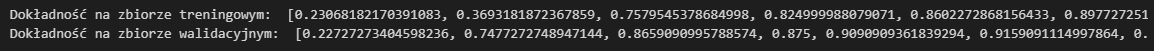
\includegraphics[width=10cm]{../thesis/resources/model/images/scr-standard-result.png}
        \caption{Przykładowe wartości dokładności dla zbioru treningowe i~walidacyjnego}
    \end{figure}
    
    \begin{figure}[ht]
        \centering
        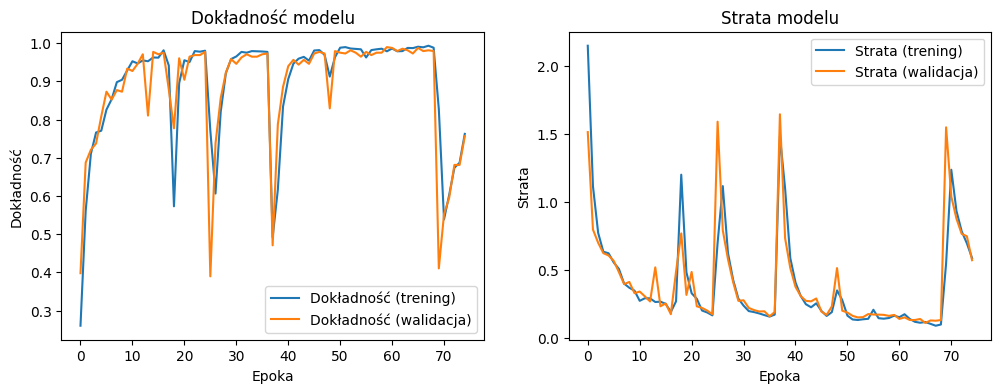
\includegraphics[height=4cm]{../thesis/resources/model/images/v2_epoch75.png}
        \caption{Przykładowa wizualizacja dokładności i~straty wytrenowanego modelu}
    \end{figure}

\end{frame}